%%%%%%%%%%%%%%%%%%%%%%%%%%%%% Define Article %%%%%%%%%%%%%%%%%%%%%%%%%%%%%%%%%%
\documentclass{article}
%%%%%%%%%%%%%%%%%%%%%%%%%%%%%%%%%%%%%%%%%%%%%%%%%%%%%%%%%%%%%%%%%%%%%%%%%%%%%%%

%%%%%%%%%%%%%%%%%%%%%%%%%%%%% Using Packages %%%%%%%%%%%%%%%%%%%%%%%%%%%%%%%%%%
\usepackage[utf8]{inputenc}
\usepackage{float, geometry, graphicx, fancyhdr, color, xcolor}
\usepackage{amssymb, amsthm, amsmath, tikz, pgfplots, comment, wrapfig}
\usepackage{listings, mdframed, lipsum, psfrag, parskip, empheq, subfig, verbatim}
\usepackage[english]{babel}
\usepackage[breaklinks]{hyperref}
\usepackage{titlesec, cite, hyperref, wrapfig, booktabs, bookmark, pdfpages}

%%%%%%%%%%%%%%%%%%%%%%%%%%%%%%%%%%%%%%%%%%%%%%%%%%%%%%%%%%%%%%%%%%%%%%%%%%%%%%%

%%%%%%%%%%%%%%%%%%%%%%%%%% C Code Listing Settings %%%%%%%%%%%%%%%%%%%%%%%%%%%%%%%%%%%%%%%
\definecolor{mGreen}{rgb}{0.25,0.63,0.15}
\definecolor{mGray}{rgb}{0.5,0.5,0.5}
\definecolor{mPurple}{rgb}{0.58,0,0.82}
\definecolor{codeBlue}{rgb}{0.01, 0.2, 0.92}
\definecolor{codegray}{rgb}{0.5,0.5,0.5}
\definecolor{codepurple}{rgb}{0.58,0,0.82}
\definecolor{codeblue}{rgb}{0.13,0.29,0.53}
\definecolor{backgroundColour}{rgb}{0.95,0.95,0.95}

\lstset{
    language=Python,
    backgroundcolor=\color{backgroundColour},
    basicstyle=\ttfamily\small,
    commentstyle=\color{deepGreen},
    keywordstyle=\color{blue},
    numberstyle=\tiny\color{mGray},
    stringstyle=\color{red},
    breakatwhitespace=false,         
    breaklines=true,                 
    captionpos=b,                    
    keepspaces=true,                 
    numbers=left,                    
    numbersep=5pt,                  
    showspaces=false,                
    showstringspaces=false,
    showtabs=false,                  
    tabsize=2,
    frame=single
}

%%%%%%%%%%%%%%%%%%%%%%%%%%%%%%%%%%%%%%%%%%%%%%%%%%%%%%%%%%%%%%%%%%%%%%%%%%%%%%%

% Other Settings
\hypersetup{
    colorlinks = true,
    linkcolor = black,
    urlcolor = blue,
}
\urlstyle{same}

%%%%%%%%%%%%%%%%%%%%%%%%%% Page Setting %%%%%%%%%%%%%%%%%%%%%%%%%%%%%%%%%%%%%%%
\geometry{a4paper}
\pagestyle{fancy}
\fancyhead{}
\fancyhead[L]{Computational Intelligence}
\fancyhead[C]{Assignment 01 - Report}
\fancyhead[R]{CS 451}
\fancyfoot{}
\fancyfoot[C]{\thepage \;of }

%%%%%%%%%%%%%%%%%%%%%%%%%% Define some useful colors %%%%%%%%%%%%%%%%%%%%%%%%%%
\definecolor{ocre}{RGB}{243,102,25}
\definecolor{mygray}{RGB}{243,243,244}
\definecolor{deepGreen}{RGB}{26,111,0}
\definecolor{shallowGreen}{RGB}{235,255,255}
\definecolor{deepBlue}{RGB}{61,124,222}
\definecolor{shallowBlue}{RGB}{235,249,255}
%%%%%%%%%%%%%%%%%%%%%%%%%%%%%%%%%%%%%%%%%%%%%%%%%%%%%%%%%%%%%%%%%%%%%%%%%%%%%%%

%%%%%%%%%%%%%%%%%%%%%%%%%% Define an orangebox command %%%%%%%%%%%%%%%%%%%%%%%%
\newcommand\orangebox[1]{\fcolorbox{ocre}{mygray}{\hspace{1em}#1\hspace{1em}}}
%%%%%%%%%%%%%%%%%%%%%%%%%%%%%%%%%%%%%%%%%%%%%%%%%%%%%%%%%%%%%%%%%%%%%%%%%%%%%%%

%%%%%%%%%%%%%%%%%%%%%%%%%%%% English Environments %%%%%%%%%%%%%%%%%%%%%%%%%%%%%
\newtheoremstyle{mytheoremstyle}{3pt}{3pt}{\normalfont}{0cm}{\rmfamily\bfseries}{}{1em}{{\color{black}\thmname{#1}~\thmnumber{#2}}\thmnote{\,--\,#3}}
\newtheoremstyle{myproblemstyle}{3pt}{3pt}{\normalfont}{0cm}{\rmfamily\bfseries}{}{1em}{{\color{black}\thmname{#1}~\thmnumber{#2}}\thmnote{\,--\,#3}}
\theoremstyle{mytheoremstyle}
\newmdtheoremenv[linewidth=1pt,backgroundcolor=shallowGreen,linecolor=deepGreen,leftmargin=0pt,innerleftmargin=20pt,innerrightmargin=20pt,]{theorem}{Theorem}[section]
\theoremstyle{mytheoremstyle}
\newmdtheoremenv[linewidth=1pt,backgroundcolor=shallowBlue,linecolor=deepBlue,leftmargin=0pt,innerleftmargin=20pt,innerrightmargin=20pt,]{definition}{Definition}[section]
\theoremstyle{myproblemstyle}
\newmdtheoremenv[linecolor=black,leftmargin=0pt,innerleftmargin=10pt,innerrightmargin=10pt,]{problem}{Problem}[section]
%%%%%%%%%%%%%%%%%%%%%%%%%%%%%%%%%%%%%%%%%%%%%%%%%%%%%%%%%%%%%%%%%%%%%%%%%%%%%%%

\title{{\huge \textbf{Habib University \\ Computational Intelligence - CS 451}}

\vspace*{5mm}
{\LARGE \textbf{Assignment 01 - Report} \\ \textbf{Evolutionary Algorithms}}
{
\includegraphics[width=0.75\linewidth]{logo.png}} \\ 
{\Large \textbf{Instructor:} Dr. Saleha Raza}}
\author{Ali Muhammad Asad - aa07190 \\ Muhammad Yousuf Uyghur - mu07486}
\date{}

\pgfplotsset{compat=1.18}

\begin{document}
\maketitle

\newpage
\tableofcontents

\newpage
\section{Question 1 - Evolutionary Algorithms}
\subsection{Genetic Algorithm Implementation}

For the genetic algorithm, a separate class called \texttt{EvolutionaryAlgorithm} was implemented, that has attributes and methods suited for our evolutionary step.

\label{params}
\subsubsection{Parameters}
The given parameters in the pdf file were tweaked and tested upon, and eventually, the following default parameters were chosen to run our tests on as they gave better results: \vspace*{-2mm} \begin{itemize}
    \item Population Size: 100 \vspace*{-2mm}
    \item Offspring Generation: 70 \vspace*{-2mm}
    \item Number of Generations: 1000 \vspace*{-2mm}
    \item Mutation Rate: 0.95 \vspace*{-2mm}
    \item Number of Iterations 10
\end{itemize}

Having a larger population size includes more diversity in our population as a larger number of chromosomes are initialized. Similarly, having a higher offpring generation means more variety of offsprings can be generated, and thus chosen to go in the next generation. The offspring count has been kept lower than the population size so as to not take too much time. The generations have been kept at 1000 to have a better reading where the values converge. Finally, having a higher mutation rate also contributes to diversity in our population, so that our problem has a lesser likelihood of being stuck at a sub-optimal solution.

\subsubsection{Parent Selection Implementation}
The \texttt{ParentSelection} method takes as argument a \texttt{selection} scheme in the form of a string, and that selection scheme is then used to select the parents that are used to create offsprings through crossover in between the two parents, followed by mutation on the selected offsprings based on the mutation rate. The code is as follows:
\begin{lstlisting}[label={parent}, caption={Parent Selection Algorithm}]
def ParentSelection(selection: str) -> None:
    selection_method = getattr(SelectionSchemes, selection)
    parents = selection_method(population, fitness_vals, Num_Offsprings)
    for i in range(0, Num_Offsprings, 2):
        child1 = crossover(parents[i], parents[i + 1])
        child2 = crossover(parents[i], parents[i + 1])
        population.append(mutate(Mutation_Rate, child1))
        population.append(mutate(Mutation_Rate, child2))
\end{lstlisting}

\subsubsection{Survival Selection Implementation}
The \texttt{SurvivalSelection} method takes as argument a \texttt{selection} scheme in the form of a string, which is then used to select the individuals that will be sent on to the next generation, based on the selection scheme. Thus, once the new offsprings have been added, this method reduces the population size back to the default setting. In my implementation, we have followed an elitism approach, which ensures that the best individual always survives to the next generation.
\begin{lstlisting}[label=survival, caption={Survival Selection Algorithm}]
def SurvivalSelection(selection: str) -> None:
    problem.population = population
    fitness_vals = problem.fitness()
    selection_method = getattr(SelectionSchemes, selection)
    new_gen = selection_method(population, fitness_vals, Population_Size - 1)
    best_individual = getBestIndividual()
    new_gen.append(best_individual)
    population = new_gen
    problem.population = population
    fitness_vals = problem.fitness()
    generation = generation + 1
\end{lstlisting}

\subsubsection{Local Search and Replace}
Additionally, another method was defined and used, \texttt{LocalSearchAndReplace}, which performs a local search around the best individual in the population. It does this by creating a mutated version of the best individual and evaluating its fitness. If the mutated individual has a higher fitness than the current best, or if its fitness is greater than or equal to the average fitness of the population, it replaces the worst individual in the population. This method can help to improve the overall fitness of the population and potentially escape from local optima. The method works as follows:
\begin{lstlisting}[label=searchandreplace, caption={Local Search and Replace Implementation}]
def LocalSearchAndReplace() -> None:
    best_individual = getBestIndividual()
    mutated_best = self.problem.mutate(1.1, best_individual)
    mutated_fitness = self.problem.fitness_helper(mutated_best)
    if mutated_fitness < getBestFitnessScore() or mutated_fitness < getAvgFitnessScore():
        worst = fitness_vals.index(getWorstFitnessScore())
        population[worst] = mutated_best
        fitness_vals[worst] = mutated_fitness
\end{lstlisting}

% \newpage
\subsection{Traveling Salesman Problem - TSP}
In my TSP Implementation, a single chromosome represents a tour that the salesman takes. It's a list of city indices, where each index represents a city. The order of indices in the list represents the order in which the cities are visited in the tour. Additonally, since each city has some coordinates, between any two cities there has to be some distance. Therefore, the fitness function simply takes a chromosome, and for every two cities in order, it finds the distance in between and adds them to a total distance variable, thus giving the total fitness of the chromosome. Since TSP is a minimizing problem, the lower the fitness score, the better the chromosome.

\subsubsection*{Initialize Population}
This method generates the initial population of tours. I first experimented with a completely random generation of tours, however, that resulted in a very high initial value of tours, and took a high number of generations to reach optimal values. Therefore, a slightly different heuristic was taken for initializing the population. For each tour in the population: \vspace*{-2mm}
\begin{itemize}
    \item With a 90\% probability, it starts with a randomly chosen city and then adds the nearest unvisited city to the tour. Therefore, its a little bit greedy, but also initializes the population with potentially good chromosomes, due to which, we start at better fitness values from the get-go. \vspace*{-2mm}
    \item With a 10\% probability, it generates a random tour by shuffling the list of all cities.
\end{itemize}

\subsubsection*{Mutation}
The mutation method, based on the mutation rate, randomly selects two points, p1 and p2, which serves as the bases for which we split our chromosome into three parts; first, middle, and end. Then the middle part is inserted back into the chromosome, but in reversed order.

\begin{lstlisting}[label=tsp_mutation, caption={Mutation Algorithm}]
def mutate(Mutation_Rate: float, Chromosome: list) -> list:
if random.random() < Mutation_Rate:
    p1 = random.randint(0, len(Chromosome)-1)
    p2 = random.randint(p1, len(Chromosome)-1)
    chrom_middle = Chromosome[p1:p2]; chrom_first = Chromosome[:p1]; chrom_end = Chromosome[p2:]
    Chromosome = chrom_first + chrom_middle[::-1] + chrom_end
return Chromosome
\end{lstlisting}

\subsubsection*{Crossover}
This method performs a crossover operation between two parent tours to generate a child tour. It randomly selects a segment from the first parent and keeps it in the child. It then fills the rest of the child with the genes from the second parent in their original order, skipping those genes that are already included in the child from the first parent. If a gene from the second parent is already included in the child, it replaces it with the corresponding gene from the first parent. If there are still duplicate genes in the child, it replaces them with the missing genes.

\begin{lstlisting}[label=tsp_crossover, caption={Crossover Algorithm}]
def crossover(parent1: list, parent2: list) -> list:
    pivot1 = random.randint(0, len(parent1)-1)
    pivot2 = random.randint(pivot1, len(parent1)-1)
    middle = parent1[pivot1:pivot2]
    first = parent2[0:pivot1]; end = parent2[pivot2:len(parent2)]
    for i in range(len(end)):
        if end[i] in middle: end[i] = parent1[pivot2 + i]
    for i in range(len(first) -1, -1, -1):
        if first[i] in middle and first[i] not in end: first[i] = parent1[i - pivot1]
    child = first + middle + end
    for i in range(len(child)):
        if child.count(child[i]) > 1:
            if parent1[i] not in child: child[i] = parent1[i]
            elif parent2[i] not in child: child[i] = parent2[i]
            else: child[i] = [x for x in parent1 if x not in child][0]
    return child
\end{lstlisting}

\subsection{Job Shop Scheduling Problem - JSSP}
In my JSSP Implementation, a single chromosome represents a sequence of operation, where each operation is a tuple of a job and a machine. The order of operations in the chromosome represents the order in which the operations are processed. The population is initialized by creating random permutations of the operations. The fitness function initliazes two dictionaries, \texttt{machineEndTimes}, and \texttt{jobEndTimes} to keep track of when a machine and job finishes its current operation. It then iterates over each operation in the chromosome. For each operation, it finds the start time, which is the maximum of the end times of the current job and the current machine. This ensures that a machine can only start a new operation after it has finished its current operation, and a job can only start a new operation on a machine after it has finished its current operation.

The end time of an operation is the start time plus the processing time. The function updates machineEndTimes and jobEndTimes with the end time.

Finally, the function returns the maximum end time across all machines, which represents the total time it takes to complete all jobs. Since we want to minimize this time.

Since JSSP is an optimizing problem where we want to reduce the time taken, the lower the fitness score, the better the chromosome.

\subsubsection*{Mutation}
The mutation method used in the implementation is an insert mutation. It randomly selects two positions in the chromosome, removes the operation at the first position, and inserts it at the second position. The mutation is performed with the provided mutation rate.

\begin{lstlisting}[label=jssp_mutation, caption={Mutation Algorithm}]
def mutate(Mutation_Rate: float, Chromosome: list) -> list:
    if random.random() < Mutation_Rate:
        p1 = random.randint(0, len(Chromosome)-1)
        p2 = random.randint(0, len(Chromosome)-1)
        while p1 == p2:
            p2 = random.randint(0, len(Chromosome)-1)
        operation = Chromosome.pop(p1)
        Chromosome.insert(p2, operation)
    return chromosome
\end{lstlisting}

\subsubsection*{Crossover}
The crossover method used in the implementation is a variant of order crossover. It randomly selects a segment from one parent and fills in the rest of the genes from the other parent in the order they appear, while ensuring that each operation appears exactly once in the child chromosome. The crossover is directly implemented using the same logic as it was for TSP above. You can refer to that pseudocode for the crossover which can also be found \hyperref[tsp_crossover]{\textcolor{red}{here}}.

\newpage
\section{Statistics and Analysis - Evolutionary Algorithms (Q1)}
The below generated plots each follow the same parameters as mentioned above in the start of the pdf in the \hyperref[params]{\textcolor{red}{Parameters}} section. In each of the scehemes, the first scheme mentioned is the Parent Scheme, and the second scheme is the Survival Selection Scheme.
\subsection{Fitness Proportion Scheme (FPS) and Random}
\begin{figure}[H]
    \centering
    \begin{tabular}{| c | c |}
        \hline
        \subfloat[TSP]{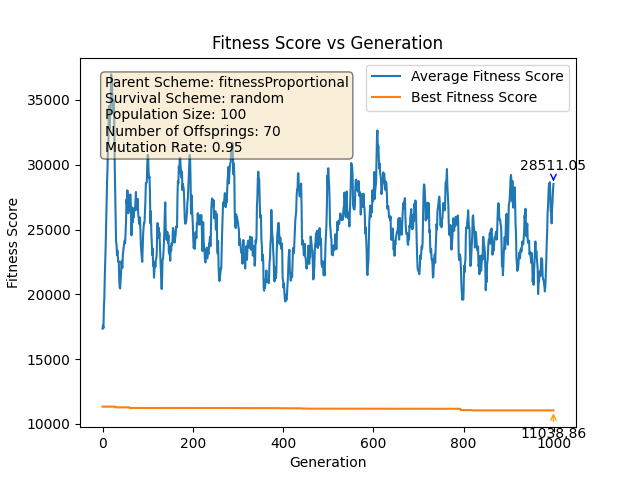
\includegraphics[width=0.475\textwidth]{Results/fps_rand/tsp_fps_rand.png}}               & \subfloat[JSSP - abz5]{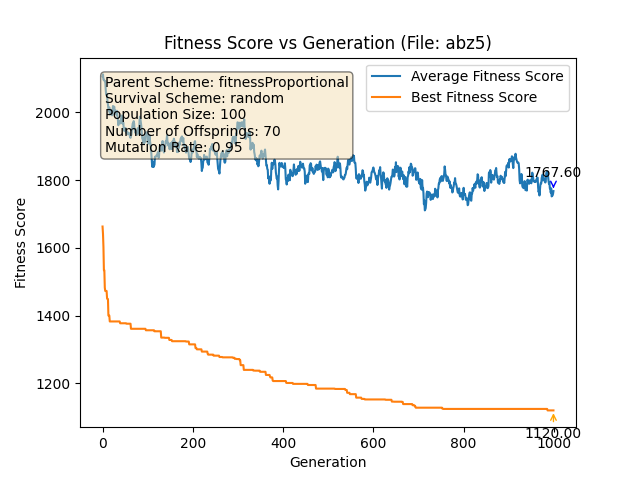
\includegraphics[width=0.475\textwidth]{Results/fps_rand/jssp_fps_rand_abz5.png}} \\ \hline
        \subfloat[JSSP - abz6]{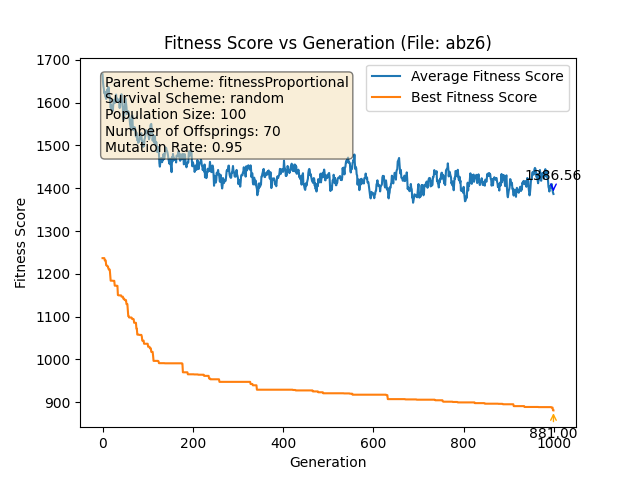
\includegraphics[width=0.475\textwidth]{Results/fps_rand/jssp_fps_rand_abz6.png}} & \subfloat[JSSP - abz7]{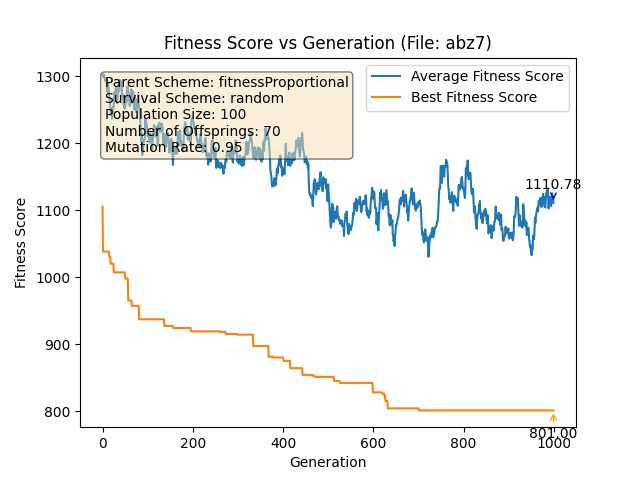
\includegraphics[width=0.475\textwidth]{Results/fps_rand/jssp_fps_rand_abz7.png}} \\ \hline
    \end{tabular}
    \begin{center}
        \caption{Plots with FPS and Random schemes}
    \end{center}
\end{figure}
As shown above, although we get a good value for the best chromosome in the population, but due to the random nature of our selection scheme, our average has a lot of variation and doesn't seem to converge towards a value, since it keeps a high diversity. Therefore, this is not a good scheme combination.

\subsection{Binary Tournament and Truncation}
\begin{figure}[H]
    \centering
    \begin{tabular}{| c | c |}
        \hline
        \subfloat[TSP]{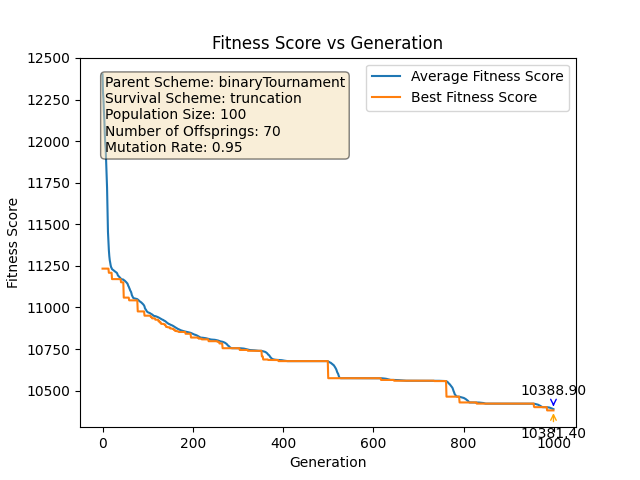
\includegraphics[width=0.475\textwidth]{Results/bin_trunc/tsp_bin_trunc.png}}               & \subfloat[JSSP - azbz5]{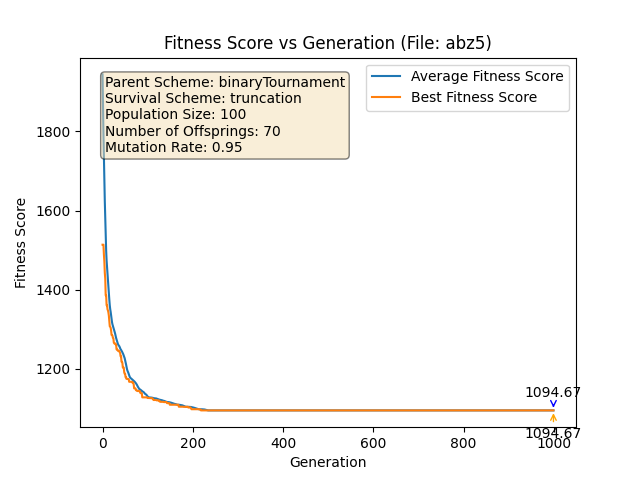
\includegraphics[width=0.475\textwidth]{Results/bin_trunc/jssp_bin_trunc_abz5.png}} \\ \hline
        \subfloat[JSSP - abz6]{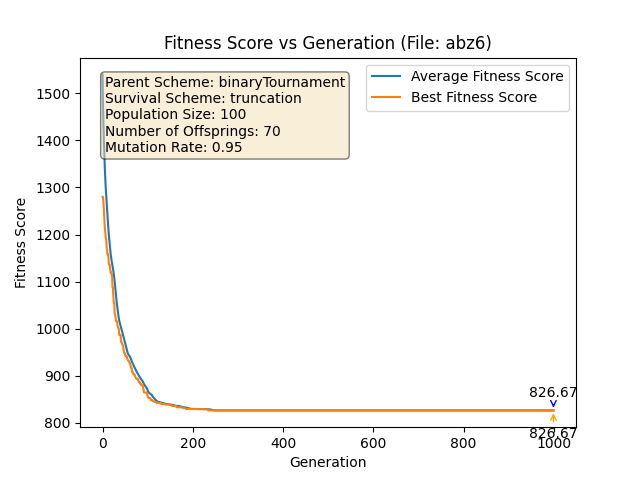
\includegraphics[width=0.475\textwidth]{Results/bin_trunc/jssp_bin_trunc_abz6.png}} & \subfloat[JSSP - abz7]{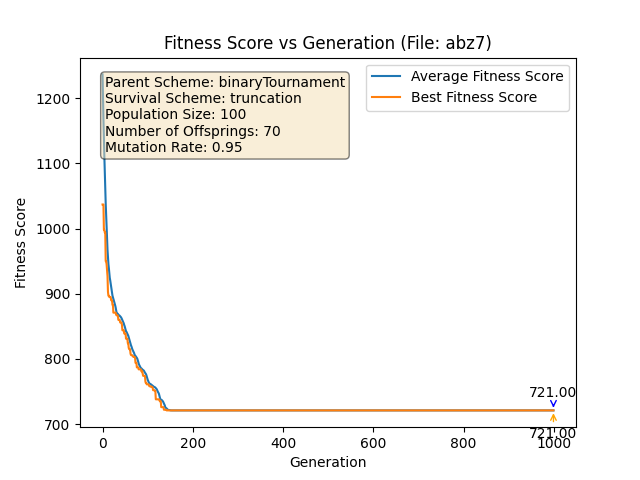
\includegraphics[width=0.475\textwidth]{Results/bin_trunc/jssp_bin_trunc_abz7.png}}  \\ \hline
    \end{tabular}
    \begin{center}
        \caption{Plots with Binary Tournament and Truncation schemes}
    \end{center}
\end{figure}

In the Binary Tournament Selection Scheme, the default tournament size has been kept as the Population Size in order to make implementation easier for us. This is a clear improvement over the previous combination scheme, as we can see the values are not only improving, but also converging towards the best value. The binary parent scheme ensures that the best parents are selected, and the truncation survival scheme ensures that only the fittest candidates move on to the next generation. This coupled with a high mutation rate ensures that there is a good balance of exploration, and exploitation in our population by including diversity as well, hence we get good values.

\subsection{Truncation and Truncation}
\begin{figure}[H]
    \centering
    \begin{tabular}{| c | c |}
        \hline
        \subfloat[TSP]{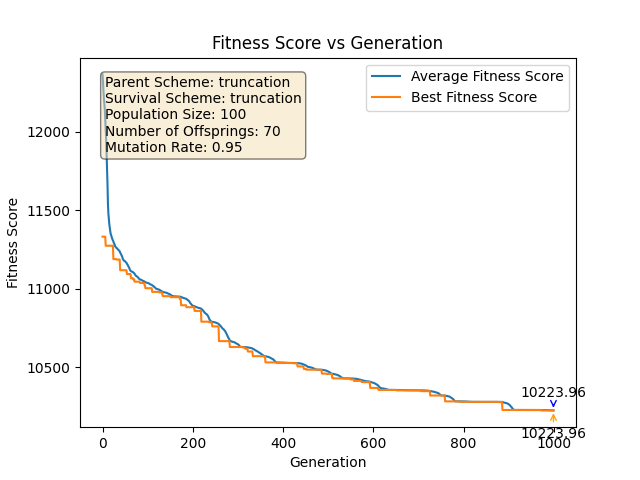
\includegraphics[width=0.475\textwidth]{Results/trunc_trunc/tsp_trunc_trunc.png}}               & \subfloat[JSSP - azbz5]{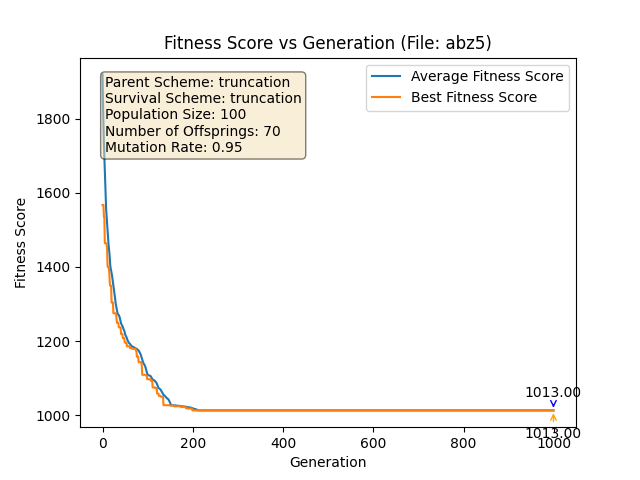
\includegraphics[width=0.475\textwidth]{Results/trunc_trunc/jssp_trunc_trunc_abz5.png}} \\ \hline
        \subfloat[JSSP - abz6]{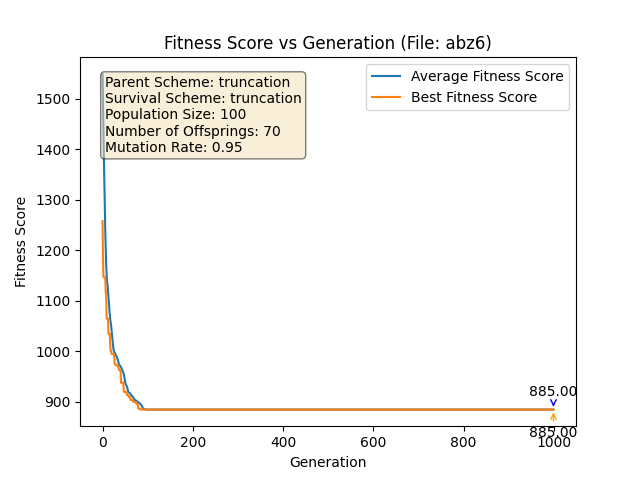
\includegraphics[width=0.475\textwidth]{Results/trunc_trunc/jssp_trunc_trunc_abz6.png}} & \subfloat[JSSP - abz7]{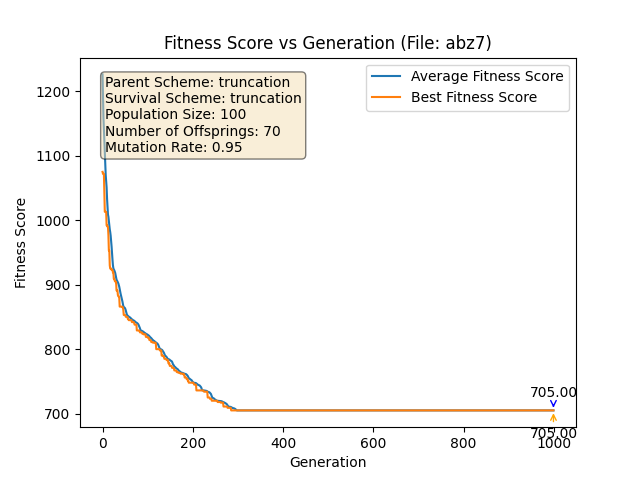
\includegraphics[width=0.475\textwidth]{Results/trunc_trunc/jssp_trunc_trunc_abz7.png}}  \\ \hline
    \end{tabular}
    \begin{center}
        \caption{Plots with Truncation scheme}
    \end{center}
\end{figure}

In this combination, since both schemes are truncation, then only the best of the chromosomes are selected as parents, and only the best of the chromosomes are selected for the next generation. This tends to be more exploitative, which can also mean that the population can quickly converge to a sub-optimal solution due to lack of diversity, therefore, a high value of exploration should be there. Our high mutation rate, and \texttt{LocalSearchAndReplace()} methods take care of this, providing a good counter to the high exploitativeness of this combination. Thus we get better results, and don't always get stuck at sub-optimal points either.

\subsection{Random and Random}
\begin{figure}[H]
    \centering
    \begin{tabular}{| c | c |}
        \hline
        \subfloat[TSP]{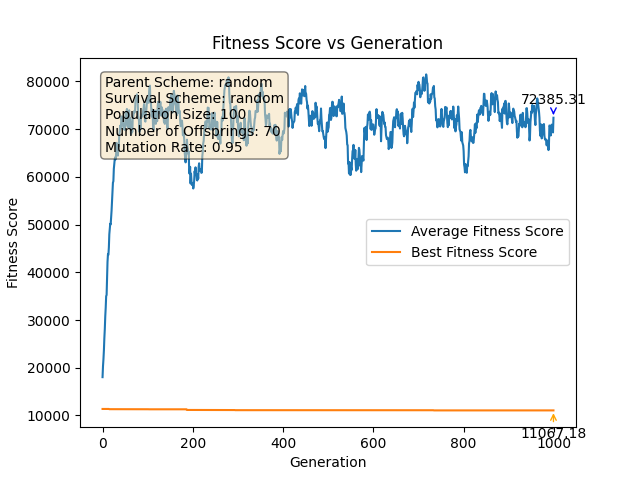
\includegraphics[width=0.475\textwidth]{Results/rand_rand/tsp_rand_rand.png}}               & \subfloat[JSSP - azbz5]{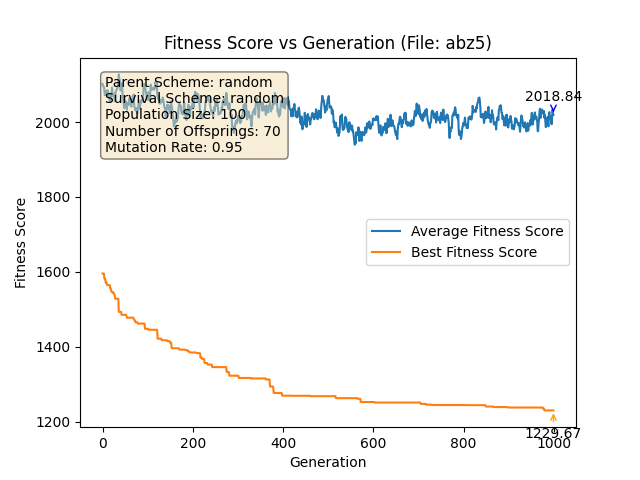
\includegraphics[width=0.475\textwidth]{Results/rand_rand/jssp_rand_rand_abz5.png}} \\ \hline
        \subfloat[JSSP - abz6]{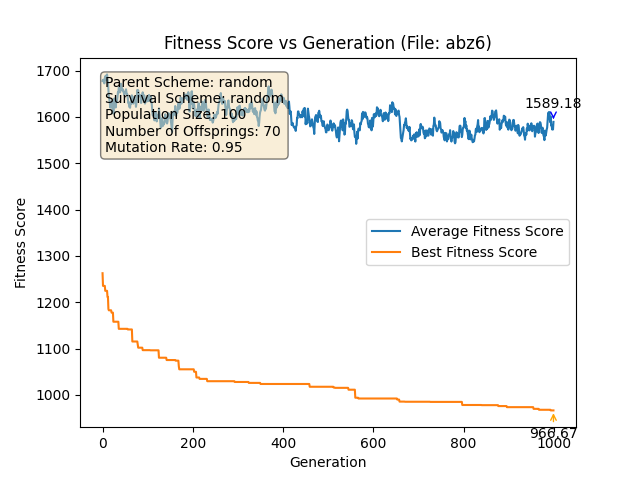
\includegraphics[width=0.475\textwidth]{Results/rand_rand/jssp_rand_rand_abz6.png}} & \subfloat[JSSP - abz7]{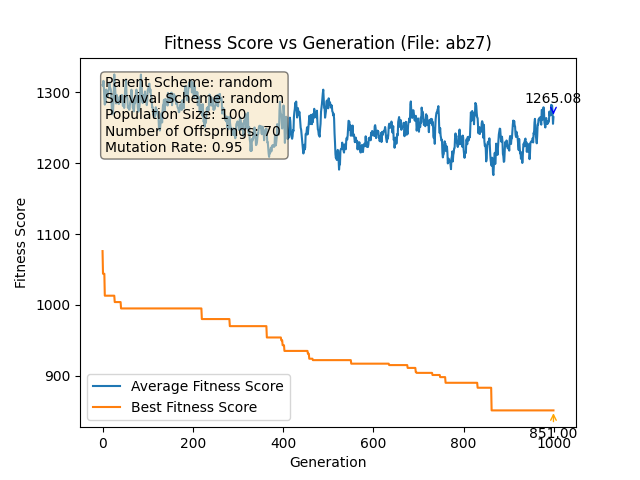
\includegraphics[width=0.475\textwidth]{Results/rand_rand/jssp_rand_rand_abz7.png}}  \\ \hline
    \end{tabular}
    \begin{center}
        \caption{Plots with Random scheme}
    \end{center}
\end{figure}

Probably the worst combination we can take, since everything is completely random, therefore, there doesn't seem to be any apparent convergence, or improvement. Rather, at some occasions our population has also gotten worse on average.

\subsection{Fitness Proportion Scheme (FPS) and Rank Based Scheme (RBS)}
\begin{figure}[H]
    \centering
    \begin{tabular}{| c | c |}
        \hline
        \subfloat[TSP]{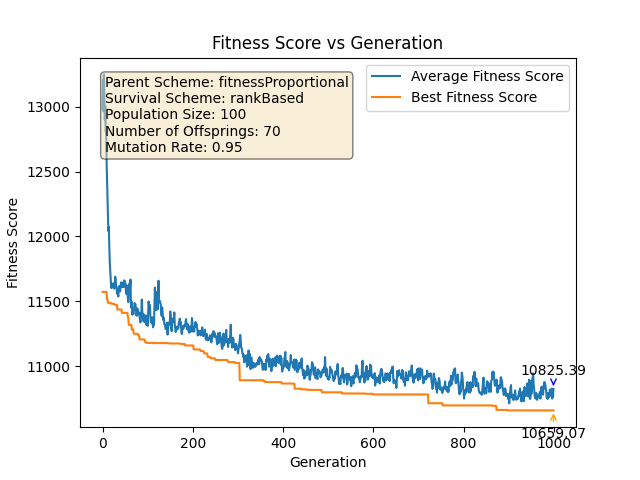
\includegraphics[width=0.475\textwidth]{Results/fps_rank/tsp_fps_rank.png}}               & \subfloat[JSSP - azbz5]{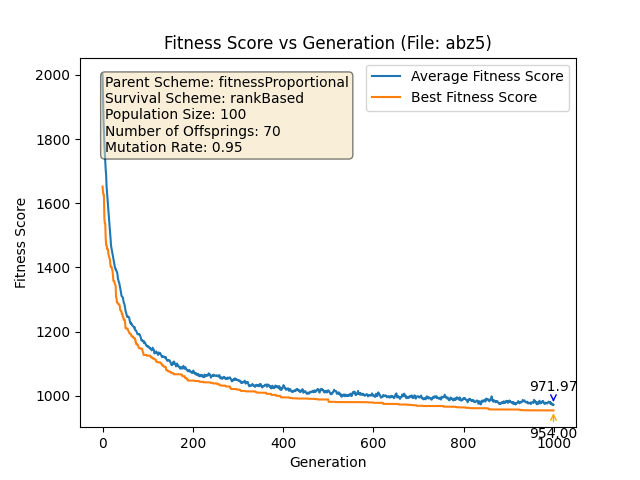
\includegraphics[width=0.475\textwidth]{Results/fps_rank/jssp_fps_rank_abz5.png}} \\ \hline
        \subfloat[JSSP - abz6]{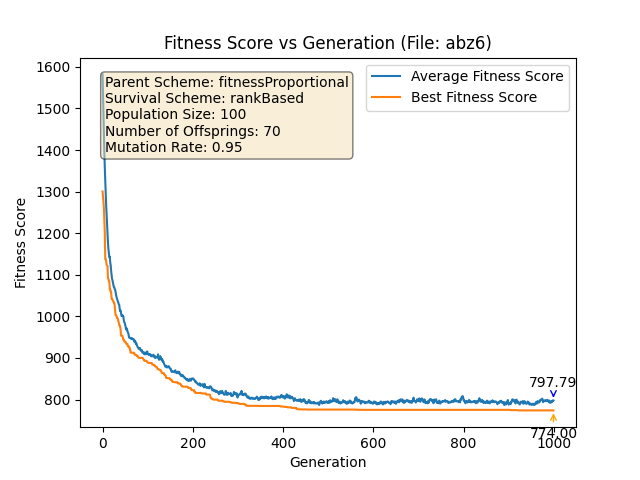
\includegraphics[width=0.475\textwidth]{Results/fps_rank/jssp_fps_rank_abz6.png}} & \subfloat[JSSP - abz7]{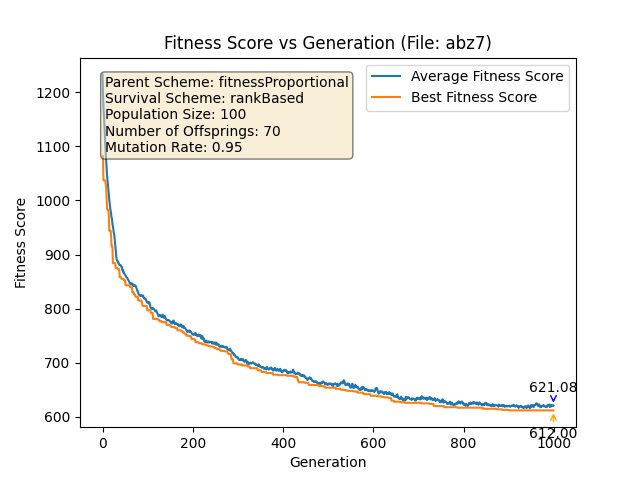
\includegraphics[width=0.475\textwidth]{Results/fps_rank/jssp_fps_rank_abz7.png}}  \\ \hline
    \end{tabular}
    \begin{center}
        \caption{Plots with FPS and Rank Based schemes}
    \end{center}
\end{figure}

Since our parents are selected proportional to their fitness, and the survivors are selected according to ranks, we see a good balance between exploration and exploitation. This also preserves diversity in our population as we can see in the varying average fitness, while also seeking better values.

\subsection{Binary Tournament and Rank Based}
\begin{figure}[H]
    \centering
    \begin{tabular}{| c | c |}
        \hline
        \subfloat[TSP]{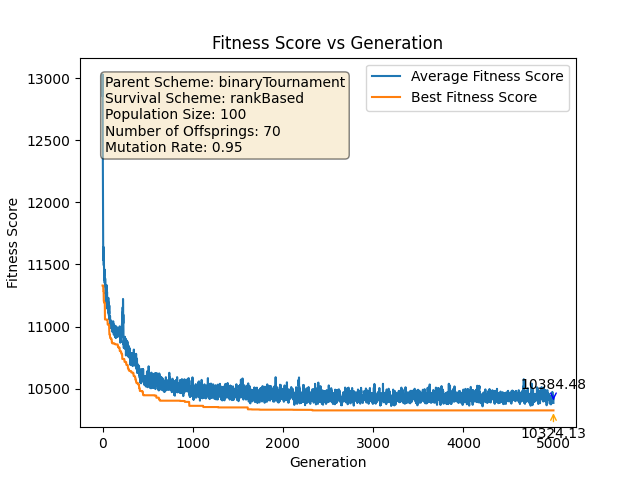
\includegraphics[width=0.475\textwidth]{Results/bin_rank/tsp_bin_rank.png}}               & \subfloat[JSSP - azbz5]{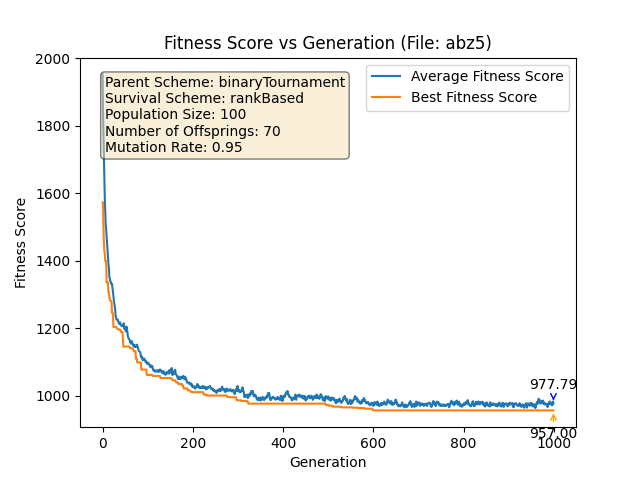
\includegraphics[width=0.475\textwidth]{Results/bin_rank/jssp_bin_rank_abz5.png}} \\ \hline
        \subfloat[JSSP - abz6]{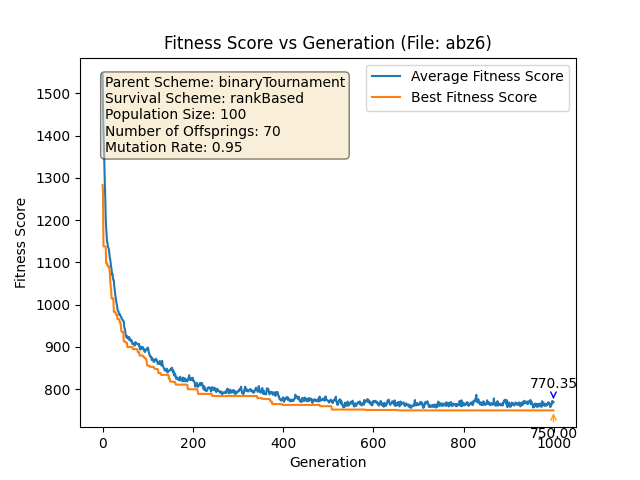
\includegraphics[width=0.475\textwidth]{Results/bin_rank/jssp_bin_rank_abz6.png}} &
        \subfloat[JSSP - abz7]{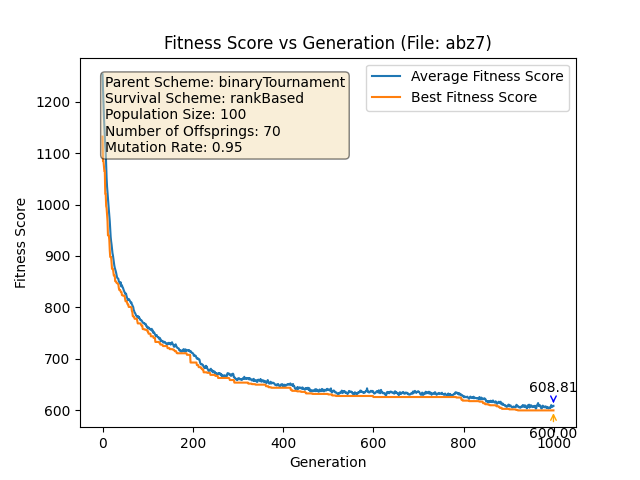
\includegraphics[width=0.475\textwidth]{Results/bin_rank/jssp_bin_rank_abz7.png}}
        \\ \hline
    \end{tabular}
    \begin{center}
        \caption{Plots with Binary Tournament and Rank Based}
    \end{center}
\end{figure}

\subsection{Rank Based and Binary Tournament}
\begin{figure}[H]
    \centering
    \begin{tabular}{| c | c |}
        \hline
        \subfloat[TSP]{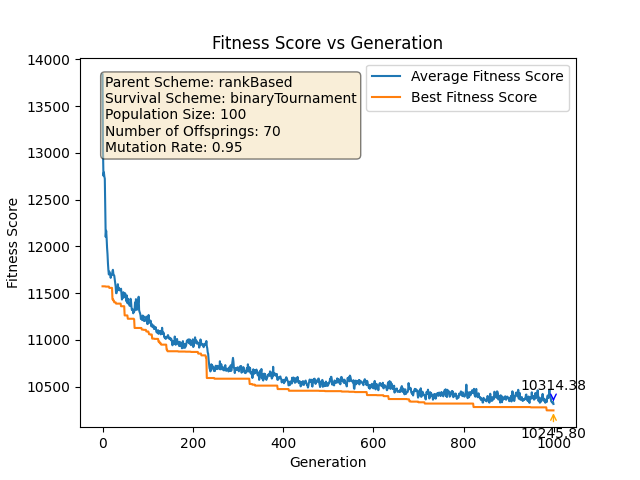
\includegraphics[width=0.475\textwidth]{Results/rank_bin/tsp_rank_bin.png}}               & \subfloat[JSSP - azbz5]{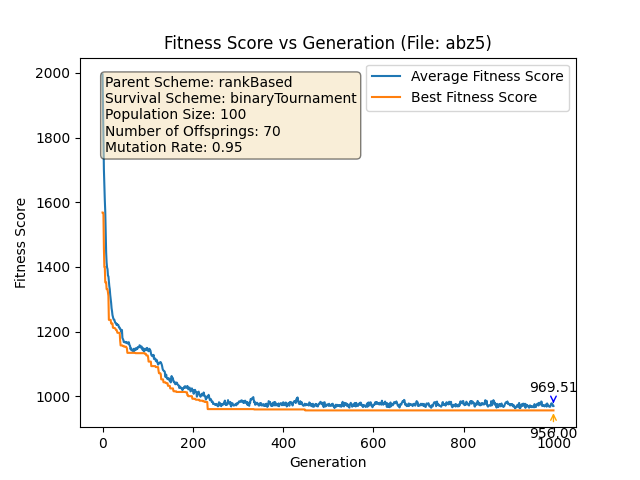
\includegraphics[width=0.475\textwidth]{Results/rank_bin/jssp_rank_bin_abz5.png}} \\ \hline
        \subfloat[JSSP - abz6]{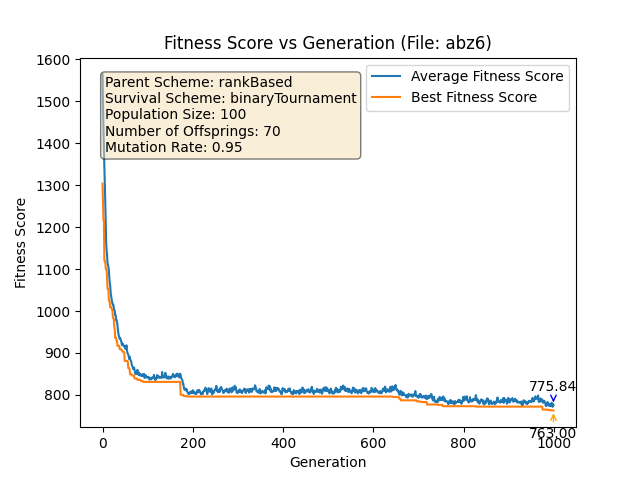
\includegraphics[width=0.475\textwidth]{Results/rank_bin/jssp_rank_bin_abz6.png}} & \subfloat[JSSP - abz7]{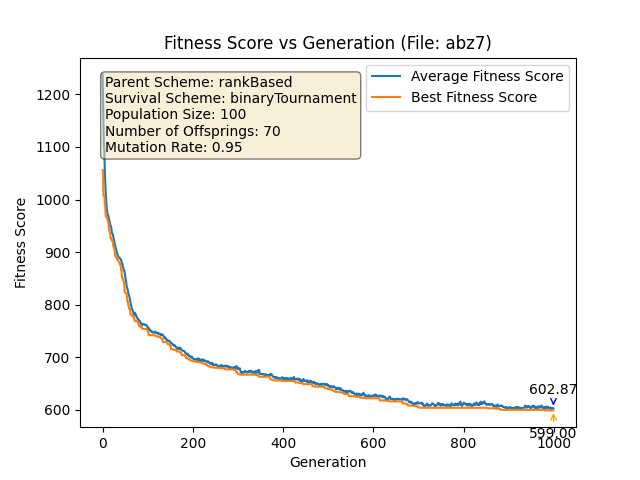
\includegraphics[width=0.475\textwidth]{Results/rank_bin/jssp_rank_bin_abz7.png}}  \\ \hline
    \end{tabular}
    \begin{center}
        \caption{Plots for Rank Based and Binary Tournament Schemes}
    \end{center}
\end{figure}

\subsection{Rank Based and Rank Based}
\begin{figure}[H]
    \centering
    \begin{tabular}{| c | c |}
        \hline
        \subfloat[TSP]{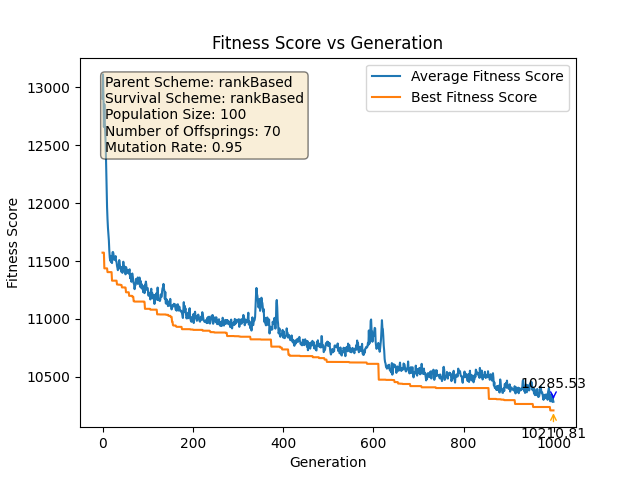
\includegraphics[width=0.475\textwidth]{Results/rank_rank/tsp_rank_rank.png}}               & \subfloat[JSSP - azbz5]{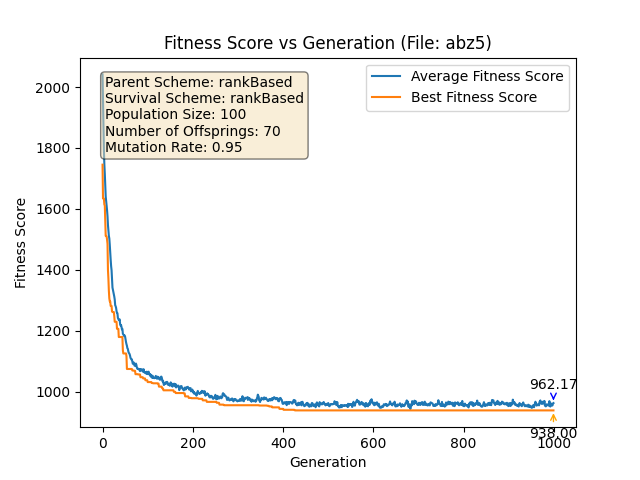
\includegraphics[width=0.475\textwidth]{Results/rank_rank/jssp_rank_rank_abz5.png}} \\ \hline
        \subfloat[JSSP - abz6]{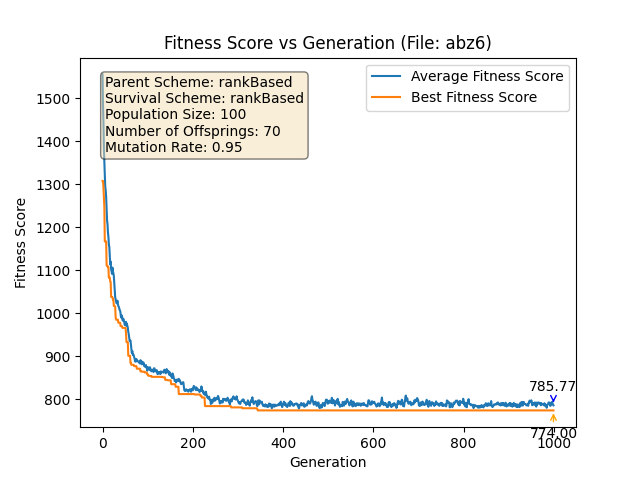
\includegraphics[width=0.475\textwidth]{Results/rank_rank/jssp_rank_rank_abz6.png}} & \subfloat[JSSP - abz7]{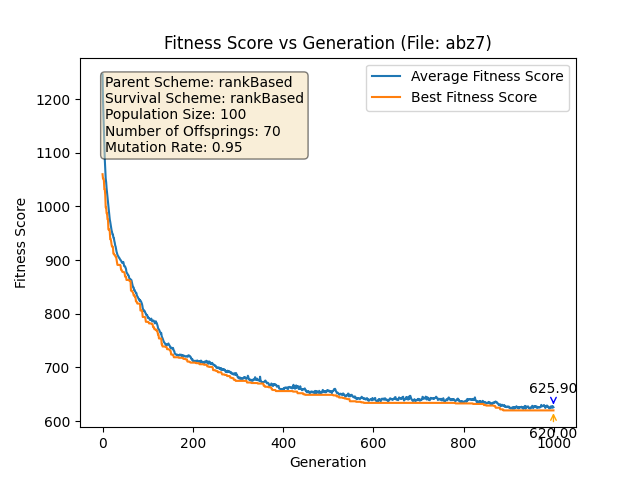
\includegraphics[width=0.475\textwidth]{Results/rank_rank/jssp_rank_rank_abz7.png}}  \\ \hline
    \end{tabular}
    \begin{center}
        \caption{Plots for Rank Based schemes}
    \end{center}
\end{figure}

\subsection{Truncation and Truncation}
\begin{figure}[H]
    \centering
    \begin{tabular}{| c | c |}
        \hline
        \subfloat[TSP]{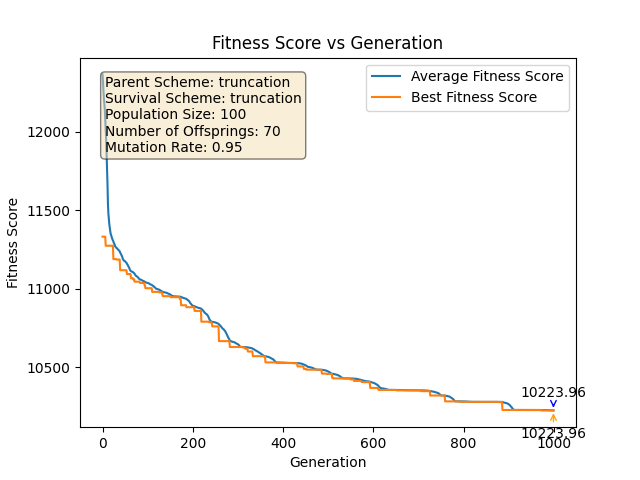
\includegraphics[width=0.475\textwidth]{Results/trunc_trunc/tsp_trunc_trunc.png}}               & \subfloat[JSSP - azbz5]{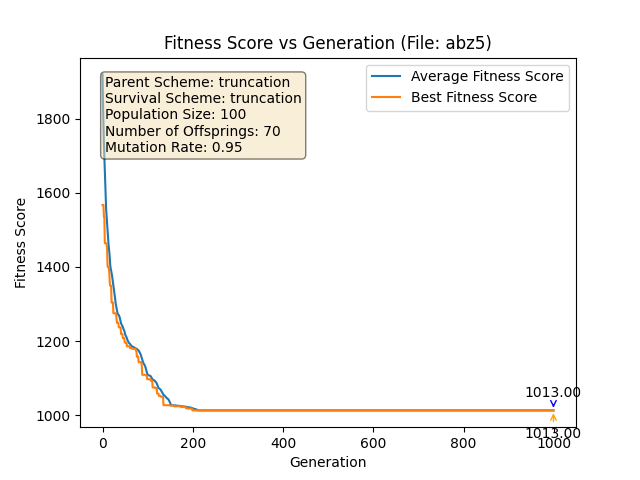
\includegraphics[width=0.475\textwidth]{Results/trunc_trunc/jssp_trunc_trunc_abz5.png}} \\ \hline
        \subfloat[JSSP - abz6]{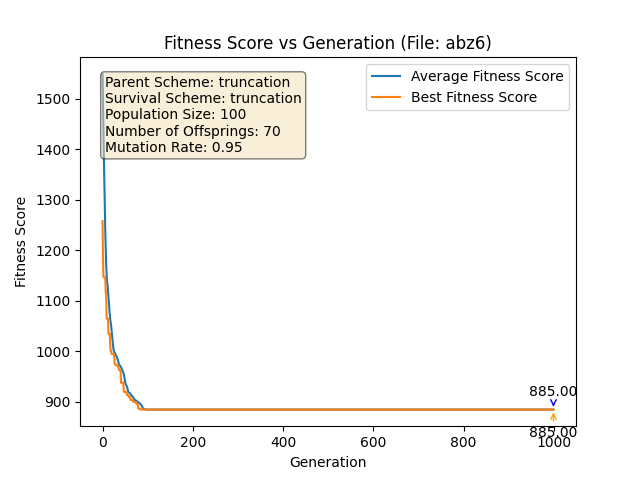
\includegraphics[width=0.475\textwidth]{Results/trunc_trunc/jssp_trunc_trunc_abz6.png}} & \subfloat[JSSP - abz7]{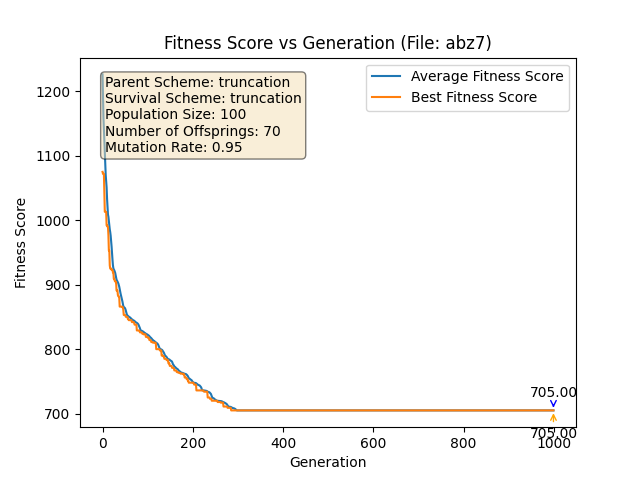
\includegraphics[width=0.475\textwidth]{Results/trunc_trunc/jssp_trunc_trunc_abz7.png}}  \\ \hline
    \end{tabular}
    \begin{center}
        \caption{Plots for Truncation schemes}
    \end{center}
\end{figure}

\subsection{Rank Based and Truncation}
\begin{figure}[H]
    \centering
    \begin{tabular}{| c | c |}
        \hline
        \subfloat[TSP]{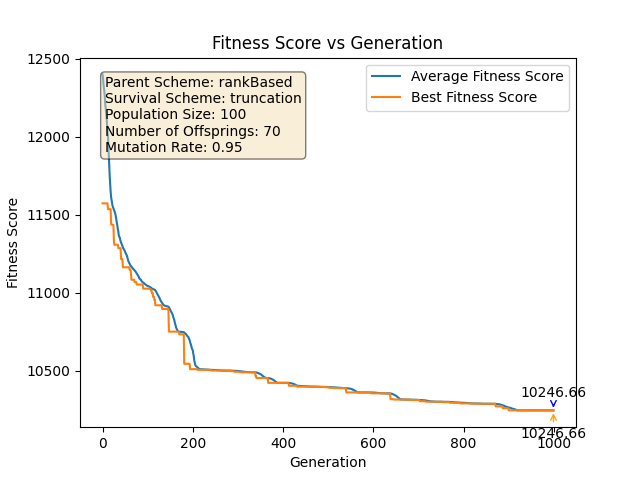
\includegraphics[width=0.475\textwidth]{Results/rank_trunc/tsp_rank_trunc.png}}               & \subfloat[JSSP - azbz5]{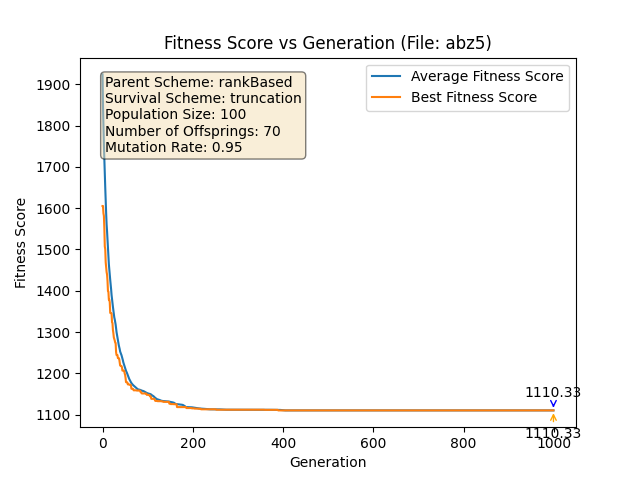
\includegraphics[width=0.475\textwidth]{Results/rank_trunc/jssp_rank_trunc_abz5.png}} \\ \hline
        \subfloat[JSSP - abz6]{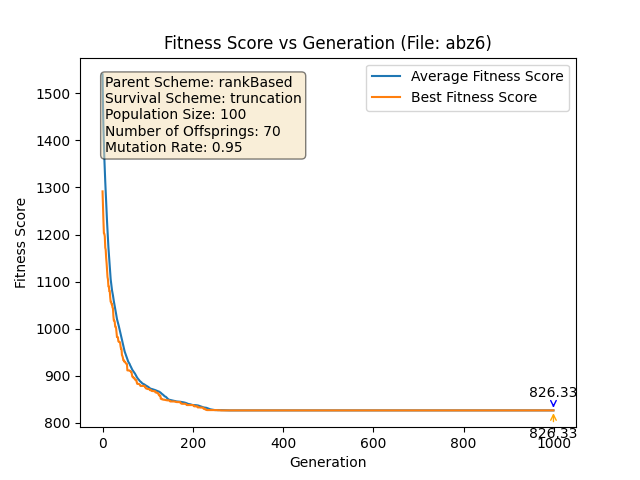
\includegraphics[width=0.475\textwidth]{Results/rank_trunc/jssp_rank_trunc_abz6.png}} & \subfloat[JSSP - abz7]{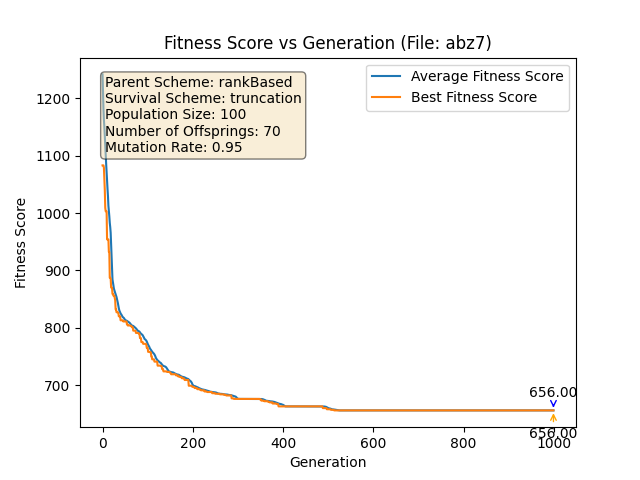
\includegraphics[width=0.475\textwidth]{Results/rank_trunc/jssp_rank_trunc_abz7.png}}  \\ \hline
    \end{tabular}
    \begin{center}
        \caption{Plots for Rank Based and Truncation Schemes}
    \end{center}
\end{figure}

% \subsection{}
% \begin{figure}[H]
%     \centering
%     \begin{tabular}{| c | c |}
%         \hline
%         \subfloat[TSP]{\includegraphics[width=0.475\textwidth]{../Results/}} & \subfloat[JSSP - azbz5]{\includegraphics[width=0.475\textwidth]{../Results/}} \\ \hline 
%         \subfloat[JSSP - abz6]{\includegraphics[width=0.475\textwidth]{../Results/}} & \subfloat[JSSP - abz7]{\includegraphics[width=0.475\textwidth]{../Results/}} \\ \hline
%     \end{tabular}
% \begin{center}
%     \caption{}
% \end{center}
% \end{figure}

\subsection{Analysis and Personal Best Values}
In those combinations where we have ``Fitness Proportion Scheme'', and ``Random Scheme'', we noticed a really high variation in our average values. Fitness still performs better, but Random introduces very high variations in our values, and hinders convergence and improvement. Therefore, after some combinations, it was decided to leave combinations involving these schemes since we already saw better results in the other combinations.

In combinations involving ``Binary Tournament'', ``Rank Based'', and ``Truncation'', we observe a lot of improvement, and convergence in our population. This is particularly true with the case of truncation, which might be due to its inherent nature of selecting those chromosomes with better fitness values. In Binary and Rank Based combinations, we can still see some variations in our average fitness, although, overall, it seems to decrease and follow the best fitness trendline, which shows that not only the best individuals are selected in each evolutionary cycle, since binary and rank based both offer diversity as they have a chance to pick other individuals apart from the best one. Due to this, they also provide a higher exploration mechanism, and less likelihood of being stuck at a sub-optimal solution. For JSSP, we see that schemes involving rank and binary tournament mostly give the best results. So does for TSP.

\subsection{Best Results for TSP}
The following images show the best results I got for TSP, on various schemes and parameters.

\begin{figure}[H]
    \centering
    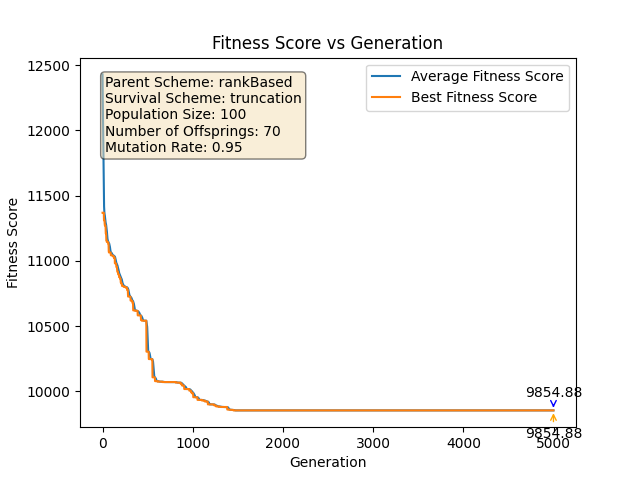
\includegraphics[width=\textwidth]{Results/noteworthy/best_tsp_rank_trunc.png}
    \caption{Best Overall TSP Score}
\end{figure}
The above image shows the best score I received for the TSP problem. For this, the following settings and parameters were used: \vspace*{-2mm} \begin{itemize}
    \item Parent Scheme: Rank Based \vspace*{-2mm}
    \item Survival Scheme: Truncation \vspace*{-2mm}
    \item Population Size: 100 \vspace*{-2mm}
    \item Offsprings: 70 \vspace*{-2mm}
    \item Mutation Rate: 0.95 \vspace*{-2mm}
    \item Initialization of Population was done greedily \vspace*{-2mm}
    \item Elitism was used in the survivor selection algorithm \vspace*{-2mm}
    \item Local Search and Replace was Implemented \vspace*{-2mm}
    \item I believe I got lucky with this run as well
\end{itemize}

The following images are also some of the best results I got, with somewhat similar settings.

\begin{figure}[H]
    \centering
    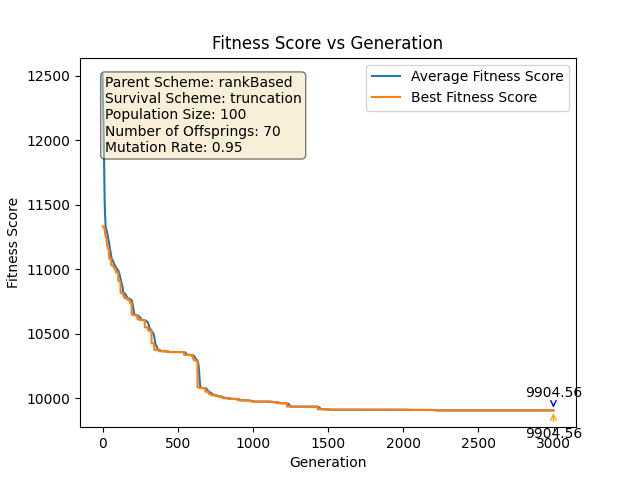
\includegraphics[width=\textwidth]{Results/noteworthy/tsp_second_best.png}
    \caption{Second Best Result}
    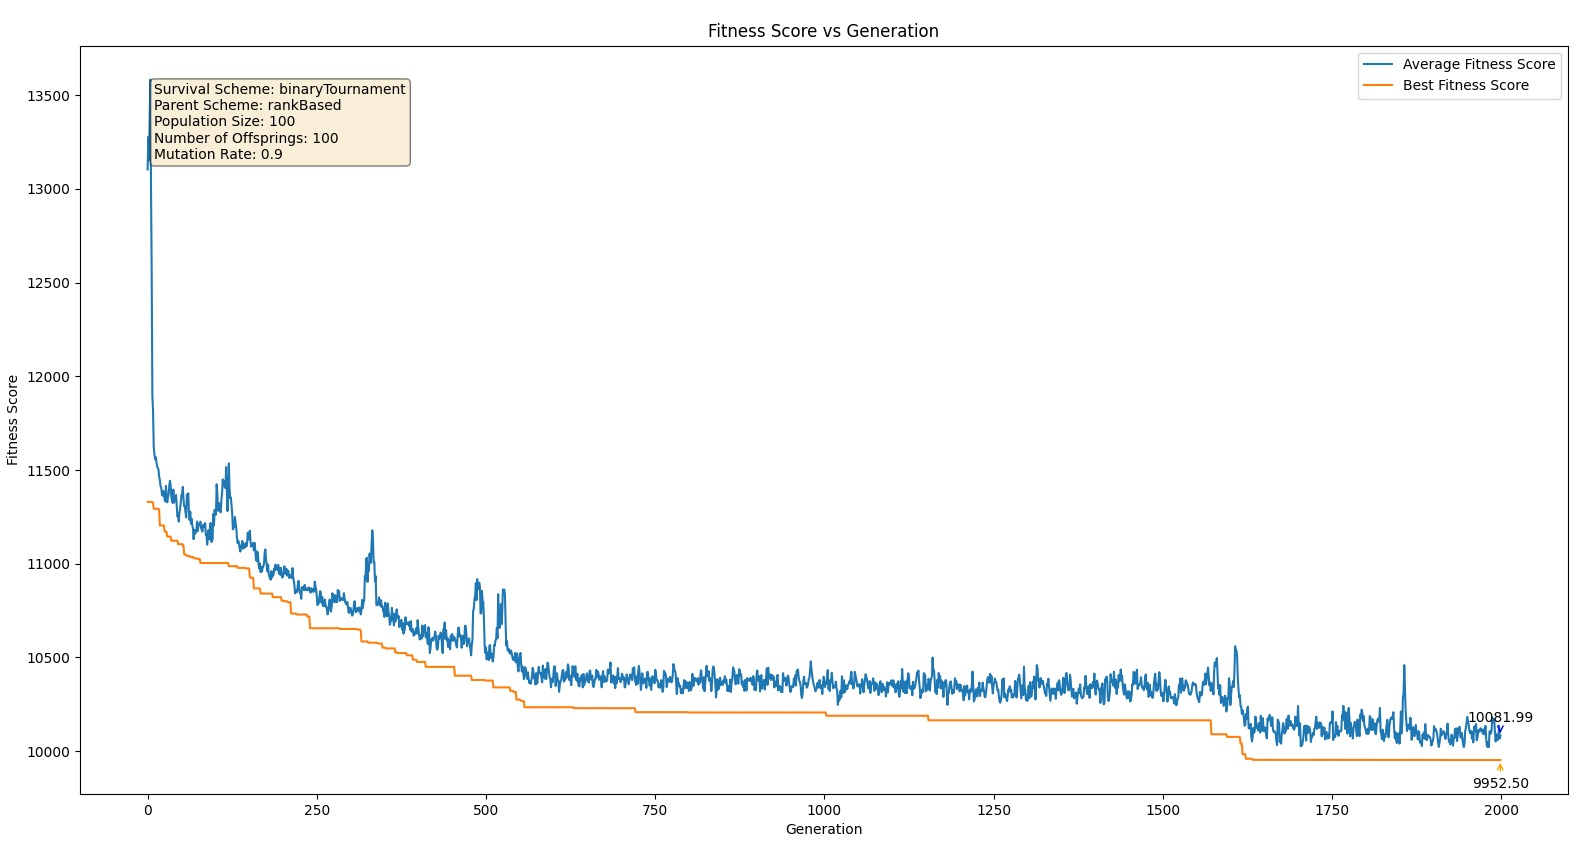
\includegraphics[width=0.9\textwidth]{Results/noteworthy/tsp_third_best.jpeg}
    \caption{Third Best Result - using Rank Based and Binary Tournament}
\end{figure}

\begin{figure}[H]
    \centering
    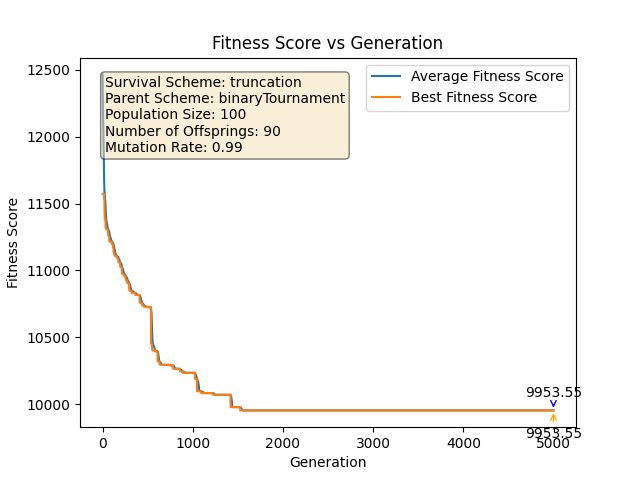
\includegraphics[width=\textwidth]{Results/noteworthy/tsp_fourth_best.png}
    \caption{Fourth Best Result - using Binary Tournament and Truncation}
\end{figure}



\newpage
\section{Evolutionary Art}


\end{document}
